% !TeX root = ../DoABook.tex


\chapter{تخمین‌های \lr{DOA} با الگوریتم‌های \lr{ESPRIT}}
\label{chap:5}

\section{مقدمه}
\label{sec:5-1}
بسیاری از الگوریتم‌هایی که تا کنون مورد بحث قرار گرفته‌اند، به دانش دقیق از ماتریس هدایت آرایه\LTRfootnote{Array steering matrix} $\bm{A}(\theta)$ وابسته هستند. برای هر $\theta_i$، پاسخ آرایه متناظر، $\bm{a}(\theta_i)$، باید مشخص باشد. این امر یا از طریق کالیبراسیون\LTRfootnote{Calibration} مستقیم در محیط واقعی و یا از طریق ابزارهای تحلیلی با استفاده از اطلاعات مربوط به موقعیت و پاسخ هر یک از عناصر مجزای آرایه به‌دست می‌آید؛ این کار معمولاً هزینه‌بر و زمان‌بر است. علاوه بر این، خطاهای کالیبراسیون ممکن است به‌طور جدی دقت تخمین را کاهش دهند. همچنین، الگوریتم‌های \lr{DOA} مبتنی بر طیف\LTRfootnote{Spectral-based} مستلزم جستجوی جامع در تمام زوایای ممکن یا تمام بردارهای هدایت برای یافتن مکان قله‌های طیفی توان و تخمین \lr{DOA} هستند که از نظر محاسباتی سنگین است.

الگوریتم \lr{ESPRIT}\LTRfootnote{Estimation of Signal Parameters via Rotational Invariance Techniques (ESPRIT)} (تخمین پارامترهای سیگنال از طریق تکنیک‌های ناورایی چرخشی) با بهره‌گیری از ویژگی ناورایی جابجایی\LTRfootnote{Shift invariance} آرایه، این مشکلات را با کاهش چشم‌گیر در نیازهای محاسباتی و حافظه برطرف می‌کند \cite{5-1}. برخلاف اکثر روش‌های تخمین \lr{DOA} مانند \lr{MUSIC}، الگوریتم \lr{ESPRIT} نیازی به دانستن دقیق بردارهای هدایت منیفولد آرایه ندارد، بنابراین الزامات کالیبراسیون آرایه در آن سخت‌گیرانه نیست. این فصل مبانی الگوریتم‌های متعلق به خانواده \lr{ESPRIT} را مرور می‌کند. بخش \ref{sec:5-1} اصل بنیادی الگوریتم‌های مبتنی بر \lr{ESPRIT} را توضیح می‌دهد. بخش \ref{sec:5-2} این اصل را برای آرایه‌های خطی یکنواخت به کار می‌گیرد. بخش \ref{sec:5-3} محاسبه زیرفضاهای سیگنال را مورد بحث قرار می‌دهد. در نهایت، در بخش‌های \ref{sec:5-4} و \ref{sec:5-5}، نسخه‌های یکانی\LTRfootnote{Unitary} الگوریتم \lr{ESPRIT} که از محاسبات با مقادیر حقیقی استفاده می‌کنند، برای فضای عنصر\LTRfootnote{Element space} و فضای پرتو\LTRfootnote{Beamspace} مورد بحث قرار می‌گیرند.

همان‌طور که در فصل \ref{chap:3} اشاره شد، یک رساله دکتری عالی در زمینه پردازش سیگنال آرایه‌ای برای تخمین‌های \lr{DOA} توسط \lr{M. Haardt} در انتشارات \textit{شاکر ورلاگ} منتشر شده است \cite{5-1}. این اثر یک بررسی و مطالعه جامع در مورد تکنیک \lr{ESPRIT} ارائه می‌دهد. به‌منظور جلوگیری از سردرگمی خواننده با نمادهای ریاضی و اصطلاحات فنی متفاوت، این فصل از همان زبان فنی و موضوعات مشابه استفاده می‌کند، در حالی که این واقعیت را نیز در نظر می‌گیرد که این نمادها و اصطلاحات در بسیاری از متون علمی مرتبط دیگر نیز به کار رفته‌اند.

\section{اصل بنیادی}
\label{sec:5-2}
در این بخش، اصل بنیادی نهفته در الگوریتم \lr{ESPRIT} توضیح داده می‌شود. \lr{ESPRIT} با اعمال یک قید بر ساختار آرایه، به کاهش پیچیدگی محاسباتی دست می‌یابد. الگوریتم \lr{ESPRIT} فرض می‌کند که یک آرایه آنتنی از دو زیرآرایه\LTRfootnote{Subarray} یکسان تشکیل شده است (شکل \ref{fig:5-1} را ببینید). زیرآرایه‌ها ممکن است دارای هم‌پوشانی باشند، یعنی یک عنصر آرایه می‌تواند عضو هر دو زیرآرایه باشد. اگر در مجموع $M$ عنصر در آرایه و $m$ عنصر در هر زیرآرایه وجود داشته باشد، هم‌پوشانی به این معناست که $M \leq 2m$. برای زیرآرایه‌هایی که هم‌پوشانی ندارند، $M = 2m$ است.

\begin{figure}[ht]
	\centering
	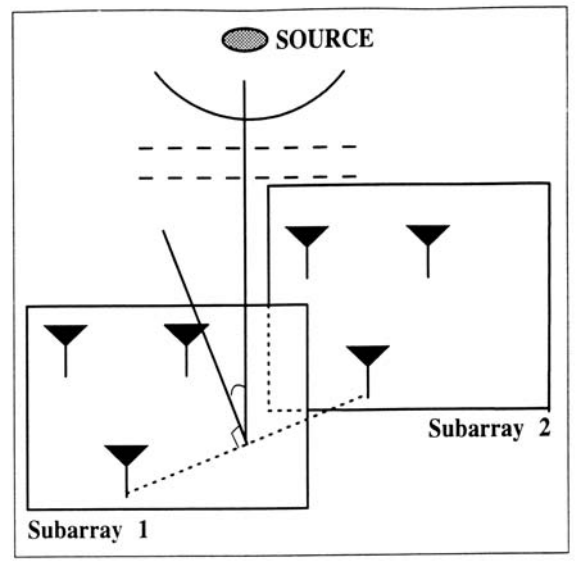
\includegraphics[width=0.8\textwidth]{chapters/figs/fig-5-1}
	\caption{ساختار آرایه آنتنی برای الگوریتم‌های مبتنی بر \lr{ESPRIT}.}
	\label{fig:5-1}
\end{figure}



عناصر منفرد هر زیرآرایه می‌توانند قطبش\LTRfootnote{Polarization}، بهره جهتی و پاسخ فاز دلخواهی داشته باشند، به شرطی که هر عنصر یک جفت یکسان در زیرآرایه همراه خود داشته باشد. فرض می‌شود عناصر هر جفت از حسگرهای یکسان، یا جفت‌حسگر\LTRfootnote{Doublet}، از نظر فیزیکی با یک بردار جابجایی\LTRfootnote{Displacement vector} ثابت (انتقالی) از هم جدا شده‌اند. بنابراین، آرایه دارای یک ناورایی جابجایی (انتقالی)\LTRfootnote{Translational invariance} است (یعنی عناصر آرایه به‌صورت جفت‌های تطبیق‌یافته با بردارهای جابجایی یکسان ظاهر می‌شوند). این ویژگی منجر به ناورایی چرخشی\LTRfootnote{Rotational invariance} زیرفضاهای سیگنال می‌شود که توسط بردارهای داده‌ی مرتبط با زیرآرایه‌های جابجا شده‌ی مکانی پوشش داده شده‌اند؛ این ناورایی سپس توسط \lr{ESPRIT} برای یافتن \lr{DOA}ها مورد استفاده قرار می‌گیرد. این مفاهیم را در بخش بعدی با جزئیات بیشتر شرح خواهیم داد.

\subsection{مدل سیگنال و داده}
\label{subsec:5-2-1}
فرض کنید $d$ سیگنال بر آرایه می‌تابند. اجازه دهید $\bm{x}_1(t)$ و $\bm{x}_2(t)$ نشان‌دهنده سیگنال‌های دریافت شده توسط دو زیرآرایه باشند که با نویز جمع‌شونده $\bm{n}_1(t)$ و $\bm{n}_2(t)$ آلوده شده‌اند. هر یک از زیرآرایه‌ها دارای $m$ عنصر هستند. با توجه به بخش \ref{subsec:3-2-1}، سیگنال‌های دریافت شده را می‌توان به‌صورت زیر بیان کرد:
\begin{subequations}
	\label{eq:5-1}
	\begin{align}
		\bm{x}_1(t) &= [\bm{a}(\mu_1), \dots, \bm{a}(\mu_d)] \bm{s}(t) + \bm{n}_1(t) = \bm{A}\bm{s}(t) + \bm{n}_1(t) \label{eq:5-1a} \\
		\bm{x}_2(t) &= [\bm{a}(\mu_1)e^{j\mu_1}, \dots, \bm{a}(\mu_d)e^{j\mu_d}] \bm{s}(t) + \bm{n}_2(t) = \bm{A}\bm{\Phi}\bm{s}(t) + \bm{n}_2(t) \label{eq:5-1b}
	\end{align}
\end{subequations}
که در آن $\bm{x}_1(t)$ و $\bm{x}_2(t)$ بردارهای $m \times 1$ هستند که داده‌های دریافت شده توسط زیرآرایه‌های اول و دوم را نشان می‌دهند. $\bm{n}_1(t)$ و $\bm{n}_2(t)$ بردارهای $m \times 1$ نشان‌دهنده نویزهای دریافت شده توسط دو زیرآرایه هستند. $\bm{A} = [\bm{a}(\mu_1), \dots, \bm{a}(\mu_d)]$ ماتریس هدایت $m \times d$ مربوط به زیرآرایه است. $\bm{s}(t)$ سیگنال‌های دریافت شده توسط زیرآرایه اول است. $\bm{\Phi} = \text{diag}[e^{j\mu_1}, \dots, e^{j\mu_d}]$ یک ماتریس قطری $d \times d$ است که سیگنال‌های دریافت شده توسط دو زیرآرایه را به هم مرتبط می‌کند و عملگر چرخش\LTRfootnote{Rotation operator} نامیده می‌شود. این عملگر ناشی از این واقعیت است که سیگنال‌های رسیده به زیرآرایه دوم، به دلیل جابجایی ثابت $\Delta$ بین دو زیرآرایه، تأخیر اضافی را تجربه می‌کنند؛ در اینجا مطابق آنچه در بخش \ref{subsec:3-2-1} توضیح داده شد، داریم:
\begin{equation}
	\mu_i = -\frac{2\pi f_c}{c} \Delta \sin \theta_i = -\frac{2\pi}{\lambda} \Delta \sin \theta_i
	\nonumber
\end{equation}

معادلات \eqref{eq:5-1a} و \eqref{eq:5-1b} را می‌توان برای تشکیل بردار خروجی کل آرایه به‌صورت زیر ترکیب کرد:
\begin{equation}
	\bm{x}(t) = \begin{bmatrix} \bm{x}_1(t) \\ \bm{x}_2(t) \end{bmatrix} = \begin{bmatrix} \bm{A} \\ \bm{A}\bm{\Phi} \end{bmatrix} \bm{s}(t) + \begin{bmatrix} \bm{n}_1(t) \\ \bm{n}_2(t) \end{bmatrix} = \tilde{\bm{A}}\bm{s}(t) + \bm{n}(t)
	\label{eq:5-2}
\end{equation}
با داشتن $N$ اسنپ‌شات $\bm{x}(t_1), \bm{x}(t_2), \dots, \bm{x}(t_N)$، هدف تکنیک \lr{ESPRIT} تخمین \lr{DOA}ها از طریق تخمین $\mu_i$ با تعیین $\bm{\Phi} = \text{diag}[e^{j\mu_1}, \dots, e^{j\mu_d}]$ است. برای انجام این کار، بر اساس داده‌های دریافت شده توسط آرایه، دو مرحله لازم است: تخمین زیرفضای سیگنال و سپس تخمین عملگر چرخش زیرفضا \cite{5-1, 5-2, 5-3}. این مراحل در بخش \ref{subsec:5-2-2} بیشتر تشریح شده‌اند.




\subsection{تخمین زیرفضای سیگنال}
\label{subsec:5-2-2}
برای یک سیگنال واحد، اگر $\bm{x}(t) = \bm{a}(\theta)s(t)$ باشد (یعنی در وضعیت ایده‌آل بدون نویز)، داده‌ها به یک زیرفضای یک‌بعدی از $\mathbb{C}^M$ محدود می‌شوند که توسط بردار هدایت $\bm{a}(\theta)$ مشخص می‌گردد. برای $d$ سیگنال، بردارهای داده‌ی مشاهده‌شده $\bm{x}(t) = \bm{As}(t)$ به یک زیرفضای $d$-بعدی از $\mathbb{C}^M$ محدود می‌شوند که زیرفضای سیگنال\LTRfootnote{Signal subspace} نامیده می‌شود (همان‌طور که در بخش \ref{sec:2-6} توصیف شد). هدف در اینجا تخمین این زیرفضای سیگنال $d$-بعدی است. فرض کنید $\bm{E}_1$ و $\bm{E}_2$ نشان‌دهنده دو مجموعه از بردارها باشند که همان زیرفضای سیگنال را پوشش می‌دهند؛ زیرفضایی که در حالت ایده‌آل توسط ستون‌های $\bm{A}$ نیز پوشش داده می‌شود. زیرفضای سیگنال را می‌توان از کوواریانس خروجی آرایه $\bm{R}_{xx}$ به‌دست آورد، همان‌طور که در بخش \ref{subsec:3-3-3} توضیح داده شد. ماتریس کوواریانس داده $\bm{R}_{xx}$ دارای فرم زیر است:
\begin{equation}
	\bm{R}_{xx} = E\{\bm{x}(t)\bm{x}^H(t)\} = \tilde{\bm{A}} \bm{R}_{ss} \tilde{\bm{A}}^H
	\label{eq:5-3}
\end{equation}
فرض می‌شود که هم $\bm{R}_{ss}$ و هم ماتریس هدایت $\tilde{\bm{A}}$ دارای رتبه کامل $d$ باشند. فرض کنید زیرفضای سیگنال به‌صورت $\bm{E}_s = [\bm{e}_1, \dots, \bm{e}_d]$ پوشش داده شود. از آنجا که $\bm{R}_{ss}$ دارای رتبه کامل است، $\bm{E}_s$ همان فضایی را پوشش می‌دهد که $\tilde{\bm{A}}$ پوشش می‌دهد. در نتیجه، باید یک ماتریس غیرتکین منحصربه‌فرد $\bm{T}$ وجود داشته باشد به‌طوری که $\bm{E}_s = \tilde{\bm{A}}\bm{T}$.

$\bm{E}_s$ را می‌توان به دو بخش $\bm{E}_1$ و $\bm{E}_2$ مربوط به دو زیرآرایه تجزیه کرد، به‌طوری که:
\begin{equation}
	\bm{E}_s = \begin{bmatrix} \bm{E}_1 \\ \bm{E}_2 \end{bmatrix} = \begin{bmatrix} \bm{AT} \\ \bm{A\Phi T} \end{bmatrix}
	\label{eq:5-4}
\end{equation}
که از آن می‌توان مشاهده کرد:
\begin{equation}
	\text{Range}\{\bm{E}_1\} = \text{Range}\{\bm{E}_2\} = \text{Range}\{\bm{A}\}
	\label{eq:5-5}
\end{equation}
معادله \eqref{eq:5-5} اساساً بیانگر این است که دو زیرآرایه، زیرفضای سیگنال یکسانی را پوشش می‌دهند و بعد یکسانی دارند؛ این امر به دلیل پیکربندی یکسان آن‌هاست. در نتیجه، یک ماتریس $d \times d$ غیرتکین که با $\bm{\Psi}$ نشان داده می‌شود را می‌توان یافت به‌طوری که:
\begin{equation}
	\bm{E}_1 \bm{\Psi} = \bm{E}_2 \Rightarrow \bm{AT\Psi} = \bm{A\Phi T}
	\label{eq:5-6}
\end{equation}
و
\begin{equation}
	\bm{\Psi} = \bm{T}^{-1} \bm{\Phi} \bm{T}
	\label{eq:5-7}
\end{equation}

همان‌طور که اکنون دیده می‌شود، $\bm{\Psi}$ و $\bm{\Phi}$ از طریق یک تبدیل تشابهی حافظ مقادیر ویژه\LTRfootnote{Eigenvalue-preserving similarity transformation} به هم مرتبط هستند. عناصر قطری (یا مقادیر ویژه) ماتریس $\bm{\Phi}$ برابر با مقادیر ویژه ماتریس $\bm{\Psi}$ هستند؛ ماتریسی که ماتریس زیرفضای سیگنال $m$-بعدی $\bm{E}_1$ (متناظر با زیرآرایه اول) را به ماتریس زیرفضای سیگنال $m$-بعدی $\bm{E}_2$ (متناظر با زیرآرایه دوم) نگاشت می‌کند (می‌چرخاند). به عبارت دیگر، ویژگی ناورایی جابجایی\LTRfootnote{Shift-invariance} اکنون بر حسب بردارهای ویژه سیگنال که زیرفضای سیگنال را پوشش می‌دهند، بیان شده است. بنابراین، در \lr{ESPRIT}، به‌جای یافتن مستقیم چرخش مکانی $\bm{\Phi}$، ما عملگر چرخش زیرفضا\LTRfootnote{Subspace rotating operator} $\bm{\Psi}$ و سپس مقادیر ویژه آن را که حاوی اطلاعات \lr{DOA} هستند، می‌یابیم.


\subsection{تخمین عملگر چرخش زیرفضا}
\label{subsec:5-2-3}
در شرایط عملی، تنها تعداد محدودی از داده‌های آلوده به نویز دریافت شده و در دسترس هستند. در این حالت، $\bm{E}_s$ از ماتریس داده $\bm{X}$ یا ماتریس کوواریانس $\bm{R}_{xx} = E[\bm{x}(t)\bm{x}^H(t)] = \tilde{\bm{A}}\bm{R}_{ss}\tilde{\bm{A}}^H + \sigma_N^2 \bm{I}_{2m}$ تخمین زده می‌شود. به دلیل وجود این نویزها، $\text{Range}\{\bm{E}_s\} \neq \text{Range}\{\tilde{\bm{A}}\}$ و $\text{Range}\{\bm{E}_1\} \neq \text{Range}\{\bm{E}_2\}$ خواهد بود. بنابراین، رابطه $\bm{E}_1 \bm{\Psi} = \bm{E}_2$ مشابه آنچه در \eqref{eq:5-6} آمد، نمی‌تواند به‌طور دقیق حل شود. از این رو، باید رویکردی برای به‌دست آوردن تخمین مناسبی از $\bm{\Psi}$ توسعه یابد. دو رویکردی که عموماً برای مسائلی از این دست به کار گرفته می‌شوند، حداقل مربعات\LTRfootnote{Least squares (LS)} \cite{5-4} و حداقل مربعات کل\LTRfootnote{Total least squares (TLS)} \cite{5-5} هستند که منجر به دو نسخه از \lr{ESPRIT} می‌شوند.

این دو رویکرد را می‌توان با در نظر گرفتن \eqref{eq:5-6} به‌عنوان یک مدل ماتریسی ساده $\bm{AX} = \bm{B}$ توضیح داد. برای تخمین $\bm{X}$، تکنیک حداقل مربعات فرض می‌کند که ماتریس $\bm{A}$ معلوم است و تمام خطاها در مسئله به نویز موجود در $\bm{B}$ نسبت داده می‌شوند. در این صورت راه حل حداقل مربعات به‌صورت زیر داده می‌شود:
\begin{equation}
	\hat{\bm{X}} = (\bm{A}^H \bm{A})^{-1} \bm{A}^H \bm{B}
	\nonumber
\end{equation}
که در آن $\hat{\bm{X}}$ تخمین $\bm{X}$ است.

با این حال، $\bm{A}$ نیز از داده‌های دریافتی حاوی نویز یا اغتشاش تعیین می‌شود و بنابراین ممکن است خود دارای خطا باشد. در نتیجه، تکنیک حداقل مربعات کل (\lr{TLS}) ترجیح داده شده و برای حل معادله ناورایی استفاده می‌شود؛ چرا که نویز را در هر دو ماتریس $\bm{A}$ و $\bm{B}$ در نظر می‌گیرد. معیار \lr{TLS} را می‌توان به‌صورت یافتن ماتریس‌های باقیمانده\LTRfootnote{Residual matrices} $\bm{R}_A$ و $\bm{R}_B$ با حداقل نُرم فروبنیوس\LTRfootnote{Frobenius norm} بیان کرد، به‌طوری که:
\begin{equation}
	(\bm{A} + \bm{R}_A)\hat{\bm{X}} = \bm{B} + \bm{R}_B
	\nonumber
\end{equation}
رویه محاسباتی واقعی برای \lr{TLS} در بسیاری از منابع علمی از جمله \cite{5-5} یافت می‌شود. به‌منظور مقایسه، هر دو رویکرد \lr{ESPRIT} در بخش‌های بعدی در نظر گرفته شده و تشریح می‌شوند.

\section{\lr{ESPRIT} استاندارد}
\label{sec:5-3}
با ارائه مفاهیم و ویژگی‌های پایه \lr{ESPRIT} در بخش‌های قبل، اکنون به توصیف الگوریتم \lr{ESPRIT} استاندارد می‌پردازیم. برای وضوح بیشتر، از آرایه خطی یکنواخت (\lr{ULA}) به‌عنوان مثالی برای تشریح رویه \lr{ESPRIT} استاندارد استفاده می‌کنیم. یک \lr{ULA} شامل $M$ عنصر را در نظر بگیرید. چند پیکربندی مختلف از آرایه که برای \lr{ESPRIT} مناسب هستند در شکل \ref{fig:5-2} نشان داده شده است.

\begin{figure}[ht]
	\centering
	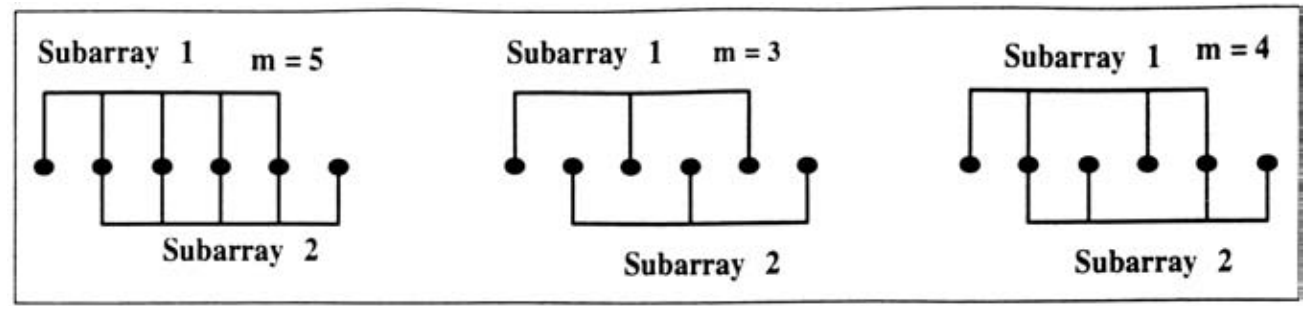
\includegraphics[width=\textwidth]{chapters/figs/fig-5-2}
	\caption{آرایه‌های خطی مرکز-متقارن و زیرآرایه‌های متناظر برای \lr{ESPRIT}.}
	\label{fig:5-2}
\end{figure}

فرض کنید دو زیرآرایه با بیشترین هم‌پوشانی\LTRfootnote{Maximum overlap} انتخاب شوند، یعنی هر زیرآرایه شامل $m = M - 1$ عنصر باشد [شکل \ref{fig:5-2}(الف) را ببینید]. ماتریس هدایت کل $\bm{A}$ برای یک \lr{ULA} دارای ساختار وندرموند زیر است:
\begin{equation}
	\bm{A} = 
	\begin{bmatrix} 
		1 & 1 & \dots & 1 \\
		e^{j\mu_1} & e^{j\mu_2} & \dots & e^{j\mu_d} \\
		\vdots & \vdots & \ddots & \vdots \\
		e^{j(M-1)\mu_1} & e^{j(M-1)\mu_2} & \dots & e^{j(M-1)\mu_d}
	\end{bmatrix}
	\label{eq:5-8}
\end{equation}
و $\bm{x}(t) = \bm{As}(t) + \bm{n}(t)$ است. هر سطر در ماتریس هدایت $\bm{A}$ متناظر با یکی از عناصر آرایه خطی است. انتخاب یک پیکربندی خاص برای زیرآرایه را می‌توان از نظر ریاضی با اعمال یک ماتریس انتخاب به ماتریس هدایت کل \eqref{eq:5-8} انجام داد؛ این ماتریس $m$ سطر از $\bm{A}$ را برمی‌گزیند.


برای مثال، یک \lr{ULA} شش‌عنصری را مطابق شکل \ref{fig:5-2} در نظر بگیرید. در حالت بیشترین هم‌پوشانی\LTRfootnote{Maximum overlap}، پنج عنصر اول زیرآرایه\LTRfootnote{Subarray} نخست و پنج عنصر آخر زیرآرایه دوم را تشکیل می‌دهند. ماتریس‌های انتخاب\LTRfootnote{Selection matrices} را می‌توان با $\bm{J}_1$، که $m = M - 1 = 5$ سطر نخست از $\bm{A}$ را برمی‌گزیند، و $\bm{J}_2$، که $m = M - 1 = 5$ سطر آخر ماتریس هدایت آرایه\LTRfootnote{Array steering matrix} $\bm{A}$ را انتخاب می‌کند، تشکیل داد. ماتریس‌های انتخاب به‌صورت زیر داده می‌شوند:
\begin{equation}
	\bm{J}_1 = [\bm{I}_m \quad \bm{0}], \quad \bm{J}_2 = [\bm{0} \quad \bm{I}_m] \in \mathbb{R}^{m \times M}
	\label{eq:5-9}
\end{equation}
که در آن $\bm{I}_m$ یک ماتریس واحد\LTRfootnote{Identity matrix} $m \times m$ است. به‌طور کلی، زیرآرایه‌ها یا به عبارتی دو ماتریس انتخاب، نسبت به یکدیگر مرکز-متقارن\LTRfootnote{Centro-symmetric} انتخاب می‌شوند؛ بدین معنا که:
\begin{equation}
	\bm{J}_2 = \bm{\Pi}_m \bm{J}_1 \bm{\Pi}_M
	\label{eq:5-10}
\end{equation}
در اینجا $\bm{\Pi}_p$ یک ماتریس تعویض\LTRfootnote{Exchange matrix} $p \times p$ است ($p = m$ یا $M$). به دلیل جابجایی\LTRfootnote{Displacement} ثابت بین زیرآرایه‌های اول و دوم، بردار هدایت زیرآرایه دوم $\bm{J}_2\bm{a}(\mu_i)$ صرفاً نسخه‌ای مقیاس‌گذاری‌شده از بردار هدایت زیرآرایه اول $\bm{J}_1\bm{a}(\mu_i)$ است:
\begin{equation}
	\bm{J}_2\bm{a}(\mu_i) = e^{j\mu_i} \bm{J}_1\bm{a}(\mu_i), \quad 1 \leq i \leq d
	\label{eq:5-11}
\end{equation}

این ویژگی ناورایی جابجایی\LTRfootnote{Shift invariance} برای تمامی $d$ بردار هدایت $\bm{a}(\mu_i)$ را می‌توان در قالب ماتریسی فشرده به‌صورت زیر بیان کرد:
\begin{equation}
	\bm{J}_1 \bm{A} \bm{\Phi} = \bm{J}_2 \bm{A}
	\label{eq:5-12}
\end{equation}
که در آن $\bm{\Phi} = \text{diag}[e^{j\mu_1}, \dots, e^{j\mu_d}]$ یک ماتریس قطری یکانی\LTRfootnote{Unitary diagonal matrix} $d \times d$ است که عناصر قطری آن حاوی اطلاعات مورد نظر \lr{DOA} در فازهای خود ($\mu_i$) هستند. الگوریتم‌های نوع \lr{ESPRIT} بر پایه این ویژگی ناورایی جابجاییِ ماتریس هدایت آرایه $\bm{A}$ بنا شده‌اند. با این حال، همان‌طور که در بخش‌های پیشین بحث شد، الگوریتم‌های \lr{ESPRIT} به‌جای یافتن مستقیم $\bm{\Phi}$، عملگر چرخش زیرفضا\LTRfootnote{Subspace rotating operator} $\bm{\Psi}$ را تخمین می‌زنند که مستقیماً با $\bm{\Phi}$ در ارتباط است. برای این منظور، همان‌گونه که در ادامه شرح داده شده است، به تخمینی از زیرفضای سیگنال\LTRfootnote{Signal subspace} نیاز است.



\subsubsection{زیرفضای سیگنال واقعی}
\label{subsec:5-3-1-1}
با توجه به این فرض که $d$ جبهه موج سیگنالِ تابیده ناهمبسته هستند (یا همان‌طور که در بخش \ref{sec:4-2} توصیف شد، «ناهمبسته شده‌اند»)، ماتریس کوواریانس سیگنال $\bm{R}_{ss} = E\{\bm{s}(t)\bm{s}^H(t)\}$ تمام‌رتبه است، یعنی $\text{rank}\{\bm{R}_{ss}\} = d$. بنابراین ماتریس کوواریانس سیگنال‌های آلوده به نویز یا داده‌ها \cite{5-4} به‌صورت زیر است:
\begin{equation}
	\bm{R}_{xx} = E\{\bm{x}(t)\bm{x}^H(t)\} = \bm{A}\bm{R}_{ss}\bm{A}^H + \sigma_N^2 \bm{I}_M \in \mathbb{C}^{M \times M}
	\label{eq:5-13}
\end{equation}

بدون نویز جمع‌شونده (یعنی $\sigma_N^2 = 0$)، ماتریس $\bm{R}_{xx}$ دچار نقص رتبه\LTRfootnote{Rank deficient} خواهد بود، زیرا:
\begin{equation}
	\text{rank}\{\bm{A}\bm{R}_{ss}\bm{A}^H\} = d < M
	\label{eq:5-14}
\end{equation}

در این حالت، $M - d$ کوچک‌ترین مقدار ویژه آن برابر با صفر هستند و تجزیه مقادیر ویژه\LTRfootnote{Eigenvalue decomposition} ماتریس $\bm{R}_{xx}$ را می‌توان به‌صورت زیر بیان کرد:
\begin{align}
	\bm{R}_{xx} \big|_{\sigma_N^2=0} &= \sum_{k=1}^{M} \lambda_k \bm{u}_k \bm{u}_k^H \nonumber \\
	&= [\bm{U}_s \quad \bm{U}_o] 
	\begin{bmatrix} 
		\bm{\Lambda}_d & \bm{0} \\
		\bm{0} & \bm{0}
	\end{bmatrix} 
	\begin{bmatrix} 
		\bm{U}_s^H \\ 
		\bm{U}_o^H 
	\end{bmatrix} = \bm{U}_s \bm{\Lambda}_d \bm{U}_s^H
	\label{eq:5-15}
\end{align}


که در آن ماتریس قطری $\bm{\Lambda}_d = \text{diag}[\lambda_1, \lambda_2, \dots, \lambda_d]$ شامل مقادیر ویژه غیرصفر است. در اینجا، مقادیر ویژه $\lambda_k$ بر اساس بزرگی‌شان مرتب شده‌اند به‌طوری که:
\begin{equation}
	\lambda_1 \geq \lambda_2 \geq \dots \geq \lambda_d > \lambda_{d+1} = \lambda_{d+2} = \dots = \lambda_M = 0
	\label{eq:5-16}
\end{equation}

ستون‌های
\begin{equation}
	\bm{U}_s = [\bm{u}_1 \quad \bm{u}_2 \ \ \ldots \ \ \bm{u}_d] \quad \text{و} \quad \bm{U}_o = [\bm{u}_{d+1} \quad \bm{u}_{d+2} \\ \ \ldots \ \ \bm{u}_M]
	\nonumber
\end{equation}
به‌ترتیب زیرفضای سیگنال $d$-بعدی $S$ و متمم متعامد\LTRfootnote{Orthogonal complement} آن را که زیرفضای نویز\LTRfootnote{Noise subspace} نامیده می‌شود، پوشش می‌دهند (همان‌طور که در بخش \ref{sec:3-6} توصیف شد). با در نظر گرفتن نویز جمع‌شونده، تجزیه مقادیر ویژه ماتریس کوواریانس $\bm{R}_{xx}$ در رابطه \eqref{eq:5-13} نتیجه می‌دهد:
\begin{align}
	\bm{R}_{xx} &= \sum_{k=1}^{M} \rho_k \bm{u}_k \bm{u}_k^H \nonumber \\
	&= [\bm{U}_s \quad \bm{U}_o] \left( 
	\begin{bmatrix} 
		\bm{\Lambda}_d & \bm{0} \\
		\bm{0} & \bm{0}
	\end{bmatrix} + \sigma_N^2 \bm{I}_M \right) 
	\begin{bmatrix} 
		\bm{U}_s^H \\ 
		\bm{U}_o^H 
	\end{bmatrix}
	\label{eq:5-17}
\end{align}

بدیهی است که با توجه به \eqref{eq:5-15} و \eqref{eq:5-17}، مقادیر ویژه $\bm{R}_{xx}$ اکنون به‌صورت $\rho_k = \lambda_k + \sigma_N^2$ برای $1 \leq k \leq d$ در می‌آیند؛ این مقادیر به اندازه $\sigma_N^2$ جابجا شده‌اند، اما بردارهای ویژه متناظر آن‌ها با بردارهای ویژه در رابطه \eqref{eq:5-15} یکسان باقی می‌مانند. از روابط \eqref{eq:5-13} و \eqref{eq:5-15} می‌توان دریافت که:
\begin{equation}
	\bm{R}_{xx} \big|_{\sigma_N^2=0} = \bm{A} \bm{R}_{ss} \bm{A}^H = \bm{U}_s \bm{\Lambda}_d \bm{U}_s^H
	\nonumber
\end{equation}

از رابطه فوق می‌توان مشاهده کرد که ستون‌های ماتریس هدایت آرایه $\bm{A}$ نیز زیرفضای سیگنال $d$-بعدی را پوشش می‌دهند، یعنی:
\begin{equation}
	S = \text{Range}\{\bm{A}\} = \text{Range}\{\bm{U}_s\}
	\label{eq:5-18}
\end{equation}

بنابراین، یک ماتریس $d \times d$ غیرتکین مانند $\bm{T}_A$ وجود دارد به‌طوری که $\bm{A} = \bm{U}_s \bm{T}_A$. از این رو، ویژگی ناورایی جابجایی در رابطه \eqref{eq:5-12} را می‌توان بر حسب بردارهای ویژه سیگنال $\bm{U}_s$ که زیرفضای سیگنال را پوشش می‌دهند، بیان کرد:
\begin{equation}
	\bm{J}_1 \bm{U}_s \bm{T}_A \bm{\Phi} = \bm{J}_2 \bm{U}_s \bm{T}_A \iff \bm{J}_1 \bm{U}_s \bm{\Psi} = \bm{J}_2 \bm{U}_s
	\label{eq:5-19}
\end{equation}



که در آن $\bm{\Psi} = \bm{T}_A^{-1} \bm{\Phi} \bm{T}_A$ یک ماتریس $d \times d$ غیرتکین و عملگر چرخش زیرفضای سیگنال است. در نتیجه، اگر زیرفضای سیگنال، که با $\bm{U}_s$ نمایش داده می‌شود، قابل تخمین باشد، می‌توان مقادیر ویژه آن را که حاوی اطلاعات \lr{DOA} هستند، یافت.

\subsubsection{تخمین زیرفضای سیگنال واقعی}
\label{subsec:5-3-1-2}
همان‌طور که پیش‌تر ذکر شد، الگوریتم \lr{ESPRIT} بر پایه تخمین زیرفضای سیگنال از ماتریس کوواریانس داده استوار است. فرض کنید $\bm{X}$ ماتریس تشکیل‌شده از داده‌های نویزآلود $N$ اسنپ‌شات $\bm{x}(t_n)$ برای $1 \leq n \leq N$ باشد:
\begin{subequations}
	\label{eq:5-20}
	\begin{align}
		\bm{X} &= [\bm{x}(t_1), \bm{x}(t_2), \dots, \bm{x}(t_N)] \nonumber \\
		&= \bm{A}[\bm{s}(t_1), \bm{s}(t_2), \dots, \bm{s}(t_N)] + [\bm{n}(t_1), \bm{n}(t_2), \dots, \bm{n}(t_N)] \nonumber \\
		&= \bm{A}\bm{S} + \bm{N} \label{eq:5-20a}
	\end{align}
	سپس تخمینی از ماتریس کوواریانس داده به‌صورت زیر به‌دست می‌آید:
	\begin{equation}
		\hat{\bm{R}}_{xx} = \frac{1}{N} \sum_{n=1}^{N} \bm{x}(t_n)\bm{x}^H(t_n) = \frac{1}{N} \bm{XX}^H \label{eq:5-20b}
	\end{equation}
\end{subequations}
زیرفضای سیگنال را می‌توان از این ماتریس کوواریانس داده تخمین زد. مطابق با رابطه \eqref{eq:5-20b} و همان‌طور که پیش‌تر مشاهده شد، بردارهای ویژه متناظر با $d$ مقدار ویژه بزرگ $\hat{\bm{R}}_{xx}$، زیرفضای سیگنال تخمینی را پوشش می‌دهند.

همان‌طور که در بخش \ref{sec:2-6-1} توصیف شد، دو رویکرد برای تخمین زیرفضای سیگنال می‌تواند مورد استفاده قرار گیرد: رویکرد کوواریانس با استفاده از تجزیه مقادیر ویژه\LTRfootnote{Eigenvalue Decomposition (EVD)} ماتریس $\bm{XX}^H$ یا رویکرد مستقیم داده با استفاده از تجزیه مقادیر منفرد\LTRfootnote{Singular Value Decomposition (SVD)} ماتریس $\bm{X}$. رویکرد اخیر نسبت به اولی این مزیت را دارد که شامل «مجذور کردن» مقادیر داده نمی‌شود. علاوه بر این، هنگام پیاده‌سازی الگوریتم روی هر پردازشگر سیگنال در زمان واقعی، باید با اعدادی با دقت محدود\LTRfootnote{Finite precision} کار کنیم؛ رویکرد کوواریانس اعدادی «بزرگ» تولید می‌کند که ممکن است منجر به مشکلات عددی مانند خطای گرد کردن\LTRfootnote{Round-off error} و سرریز\LTRfootnote{Overflow} شود. در نتیجه، رویکرد مستقیم داده ترجیح داده می‌شود؛ در این صورت \lr{SVD} ماتریس داده $\bm{X}$ به‌صورت زیر خواهد بود:
\begin{equation}
	\bm{X} = \bm{U}\bm{\Sigma}\bm{V}^H = [\bm{U}_s \quad \bm{U}_o] 
	\begin{bmatrix} 
		\bm{\Sigma}_s & \bm{0} \\
		\bm{0} & \bm{\Sigma}_o
	\end{bmatrix} 
	\begin{bmatrix} 
		\bm{V}_s^H \\ 
		\bm{V}_o^H 
	\end{bmatrix}
	\label{eq:5-21}
\end{equation}
که در آن ماتریس قطری $\bm{\Sigma}_s \in \mathbb{R}^{d \times d}$ شامل $d$ بزرگ‌ترین مقدار منفرد است و $\bm{U}_s$ زیرفضای سیگنال را پوشش می‌دهد.

\subsection{حل معادله ناورایی}
\label{subsec:5-3-2}
پس از تخمین ماتریس $\bm{U}_s$ که زیرفضای سیگنال تخمینی را پوشش می‌دهد، بر اساس رابطه \eqref{eq:5-19}، دو ماتریس انتخاب معلوم $\bm{J}_1$ و $\bm{J}_2$ برای تشکیل معادله ناورایی زیر به کار می‌روند:
\begin{equation}
	\bm{J}_1 \bm{U}_s \bm{\Psi} \approx \bm{J}_2 \bm{U}_s, \quad \bm{\Psi} \in \mathbb{C}^{d \times d}
	\label{eq:5-22}
\end{equation}
که در آن $\bm{\Psi}$ عملگر چرخش زیرفضای سیگنال است که در روابط \eqref{eq:5-6} یا \eqref{eq:5-17} تعریف شد. برعکسِ رابطه \eqref{eq:5-19}، این معادله ناورایی ممکن است راه حل دقیقی نداشته باشد؛ زیرا زیرفضای سیگنال از یک ماتریس کوواریانس داده‌ی تخمینی (رابطه \ref{eq:5-21}) استخراج شده است که ماتریس کوواریانس واقعی یا دقیق سیگنال نیست. همچنین، برای محاسبه تمام \lr{DOA}ها، اندازه زیرآرایه‌ها ($M-1$) باید حداقل برابر با $d$ باشد؛ در غیر این صورت، سیستم ناورایی \eqref{eq:5-22} کم‌معین\LTRfootnote{Underdetermined} خواهد بود.

معادله \eqref{eq:5-22} با استفاده از روش‌های حداقل مربعات (\lr{LS}) یا حداقل مربعات کل (\lr{TLS}) برای به‌دست آوردن تخمینی از عملگر چرخش زیرفضا حل می‌شود. در پیاده‌سازی این راهکارها در زمان واقعی، ممکن است از الگوریتم کارآمدتری به نام تجزیه \lr{QR}\LTRfootnote{QR decomposition} نیز برای حل حداقل مربعات استفاده شود. دلیل این امر آن است که محاسبات مستقیم معکوس ماتریس مستعد خطا بوده و زمان زیادی را در محاسبات مصرف می‌کنند \cite{5-5}.

\subsection{فرکانس مکانی و تخمین \lr{DOA}}
\label{subsec:5-3-3}
پس از یافتن $\bm{\Psi} \in \mathbb{C}^{d \times d}$، اطلاعات \lr{DOA} مورد نظر را می‌توان از روی آن تخمین زد. مقادیر ویژه $\bm{\Psi}$ تخمینی را می‌توان از طریق تجزیه مقادیر ویژه آن محاسبه کرد؛ زیرا:
\begin{equation}
	\bm{\Psi} = \bm{T}^{-1} \bm{\Phi} \bm{T} \quad \text{که در آن} \quad \bm{\Phi} = \text{diag}[e^{j\mu_1}, \dots, e^{j\mu_d}]
	\label{eq:5-23}
\end{equation}
بنابراین، مقدار ویژه $\bm{\Psi}$ که با $\phi_i$ نشان داده می‌شود، بیانگر تخمینی از فاکتورهای فاز $e^{j\mu_i}$ است. پس از یافتن تخمین‌های فرکانس مکانی $\mu_i$، زوایای \lr{DOA} متناظر ($\theta_i$) از طریق روابط زیر به‌دست می‌آیند:
\begin{equation}
	\mu_i = \arg(\phi_i) \quad \text{و} \quad \theta_i = \arcsin \left( \frac{\lambda \mu_i}{2\pi \Delta} \right), \quad 1 \leq i \leq d
	\label{eq:5-24}
\end{equation}

خلاصه‌ای از مراحل محاسباتی \lr{ESPRIT} استاندارد در جدول \ref{tab:5-1} نشان داده شده است \cite{5-1}. همان‌طور که از جدول \ref{tab:5-1} پیداست، محاسبات \lr{ESPRIT} استاندارد شامل عملیات اعداد مختلط است. برای اجتناب از این امر، نسخه‌ی بهبودیافته‌ای از \lr{ESPRIT} که تنها از محاسبات با مقادیر حقیقی استفاده می‌کند، توسعه یافته است که در بخش \ref{sec:5-4} توصیف می‌شود.


\section{تبدیل با مقادیر حقیقی}
\label{sec:5-4}
الگوریتم \lr{ESPRIT} استاندارد در تمامی مراحل خود شامل محاسبات با مقادیر مختلط\LTRfootnote{Complex-valued computations} است. این امر موجب می‌شود الگوریتم از نظر محاسباتی پرهزینه باشد. با این حال، مشاهده شده است که در صورت استفاده از آرایه‌های مرکز-متقارن، زیرفضای سیگنال را می‌توان از طریق محاسبات با مقادیر حقیقی\LTRfootnote{Real-valued computations} تخمین زد. بهره‌گیری از این ویژگی برای آرایه‌های مرکز-متقارن منجر به ظهور الگوریتم \lr{Unitary ESPRIT} می‌شود که صرفاً از محاسبات حقیقی استفاده می‌کند. بنابراین، آرایه‌های مرکز-متقارنی که در فصل \ref{chap:2} معرفی شدند، برای پیاده‌سازی \lr{Unitary ESPRIT} ضروری هستند. الگوریتم \lr{Unitary ESPRIT} بر پایه قضیه زیر فرمول‌بندی و بنا شده است \cite{5-5}.


\begin{table}[ht]
	\centering
	\caption{خلاصه‌ی الگوریتم \lr{ESPRIT} استاندارد.}
	\label{tab:5-1}
	\begin{tabular}{|p{0.9\textwidth}|}
		\hline
		\begin{enumerate}
			\item \textbf{تخمین زیرفضای سیگنال:} محاسبه‌ی $\bm{U}_s$ به‌عنوان $d$ بردار منفرد چپ غالب از $\bm{X}$ (رویکرد ریشه دوم) یا $d$ بردار ویژه‌ی غالب از $\bm{XX}^H$ (رویکرد کوواریانس).
			\item \textbf{حل معادله‌ی ناورایی:} حل معادله‌ی زیر برای $\bm{\Psi}$:
			\begin{equation*}
				\bm{J}_1 \bm{U}_s \bm{\Psi} \approx \bm{J}_2 \bm{U}_s
			\end{equation*}
			با استفاده از تکنیک‌های حداقل مربعات\LTRfootnote{Least-squares} یا حداقل مربعات کل\LTRfootnote{Total least-squares}.
			\item \textbf{تخمین \lr{DOA}:} محاسبه‌ی مقادیر ویژه‌ی راه حل مختلط حاصل:
			\begin{equation*}
				\bm{\Psi} = \bm{T}\bm{\Phi}\bm{T}^{-1} \quad \text{با} \quad \bm{\Phi} = \text{diag}[\phi_1, \dots, \phi_d]
			\end{equation*}
			و سپس استخراج اطلاعات زاویه‌ای از طریق:
			\begin{equation*}
				\begin{aligned}				\mu_i &= \arg(\phi_i), \quad 1 \leq i \leq d \\
					\theta_i &= \arcsin\left( -\frac{\lambda}{2\pi \Delta} \mu_i \right)
				\end{aligned}
			\end{equation*}
		\end{enumerate} \\
		\hline
	\end{tabular}
\end{table}

\begin{theorem}
	فرض کنید $\bm{Q}_p$ و $\bm{Q}_q$ به‌ترتیب نشان‌دهنده ماتریس‌های حقیقی-چپ-$\Pi$ با ابعاد $p \times p$ و $q \times q$ باشند که در رابطه \eqref{eq:3-16} تعریف شدند. در این صورت، برای هر ماتریس مرکز-هرمیتی $p \times q$ مانند $\bm{G}$، ماتریس $\bm{Q}_p^{-1} \bm{G} \bm{Q}_q$ یک ماتریس با مقادیر حقیقی در ابعاد $p \times q$ است.
\end{theorem}

ماتریس داده‌های بسط‌یافته تعریف‌شده در رابطه \eqref{eq:4-8} را در نظر بگیرید. این رابطه برای دسترسی سریع در اینجا بازنویسی شده است:
\begin{equation}
	\bm{Z} = [\bm{X} \quad \bm{\Pi}_M \bar{\bm{X}}]
	\label{eq:5-25}
\end{equation}
می‌توان نشان داد که $\bm{Z}$ مرکز-هرمیتی\LTRfootnote{Centro-Hermitian} است \cite{5-6}. همچنین، مشابه آنچه در بخش \ref{sec:4-2} توصیف شد، تخمین $\hat{\bm{R}}_{xx}^{fb}$ از ماتریس کوواریانس میانگین‌گیری‌شده‌ی رفت‌وبرگشت نیز مرکز-هرمیتی است \cite{5-6}:
\begin{equation}
	\hat{\bm{R}}_{xx}^{fb} = \frac{1}{2} (\hat{\bm{R}}_{xx} + \bm{\Pi}_M \hat{\bar{\bm{R}}}_{xx} \bm{\Pi}_M)
	\label{eq:5-26}
\end{equation}

اکنون، تبدیل یکانی\LTRfootnote{Unitary transformation} ماتریس داده با مقادیر مختلط به ماتریسی با مقادیر حقیقی را می‌توان با اعمال قضیه \ref{chap:5}.1 بر ماتریس داده‌های بسط‌یافته به‌دست آورد:
\begin{equation}
	\bm{\Gamma}(\bm{X}) = \bm{Q}_M^H \bm{Z} \bm{Q}_{2N} = \bm{Q}_M^H [\bm{X} \quad \bm{\Pi}_M \bar{\bm{X}}] \bm{Q}_{2N} \in \mathbb{R}^{M \times 2N}
	\label{eq:5-27}
\end{equation}

بنابراین، تبدیل $\bm{\Gamma}(\bm{X})$ میانگین‌گیری رفت‌وبرگشت را ابتدا با بسط ماتریس داده‌های مختلط $\bm{X}$ با ابعاد $M \times N$ به یک ماتریس مرکز-هرمیتی مختلط $\bm{Z}$ با ابعاد $M \times 2N$ و سپس تبدیل $\bm{Z}$ به یک ماتریس با مقادیر حقیقی با همان ابعاد، محقق می‌سازد. در نتیجه، می‌توانیم بنویسیم:
\begin{align}
	\bm{\phi} &= \bm{Q}_M^H \hat{\bm{R}}_{xx}^{fb} \bm{Q}_M \nonumber \\
	&= \frac{1}{2} \bm{Q}_M^H (\hat{\bm{R}}_{xx} + \bm{\Pi}_M \hat{\bar{\bm{R}}}_{xx} \bm{\Pi}_M) \bm{Q}_M \nonumber \\
	&= \frac{1}{2} (\bm{Q}_M^H \hat{\bm{R}}_{xx} \bm{Q}_M + \bm{Q}_M^H \bm{\Pi}_M \hat{\bar{\bm{R}}}_{xx} \bm{\Pi}_M \bm{Q}_M) \nonumber \\
	&= \frac{1}{2} (\bm{Q}_M^H \hat{\bm{R}}_{xx} \bm{Q}_M + \bar{\bm{Q}}_M^H \hat{\bar{\bm{R}}}_{xx} \bar{\bm{Q}}_M) \nonumber \\
	&= \text{Re}\{\bm{Q}_M^H \hat{\bm{R}}_{xx} \bm{Q}_M\} \in \mathbb{R}^{M \times M}
	\label{eq:5-28}
\end{align}

همان‌طور که مشاهده می‌شود، میانگین‌گیری رفت‌وبرگشت را می‌توان به‌صورت خودکار و ضمنی با گرفتن بخش حقیقی ماتریس کوواریانس تبدیل‌یافته‌ی $\bm{Q}_M^H \hat{\bm{R}}_{xx} \bm{Q}_M$ به‌دست آورد. از این رو، زیرفضای سیگنال با مقادیر حقیقی $\bm{E}_s$ را می‌توان به‌عنوان $d$ بردار منفرد چپِ غالب از $\bm{\Gamma}(\bm{X}) \in \mathbb{R}^{M \times 2N}$ (رویکرد داده مستقیم) یا $\bm{\Gamma}(\bm{X})\bm{\Gamma}(\bm{X})^H \in \mathbb{R}^{M \times M}$ (رویکرد کوواریانس) یافت. این اصل برای فرمول‌بندی نسخه جدیدی از \lr{ESPRIT} به نام \lr{Unitary ESPRIT} به کار گرفته می‌شود که در ادامه توصیف می‌گردد.

\section{الگوریتم \lr{Unitary ESPRIT} در فضای عنصر}
\label{sec:5-5}
الگوریتم \lr{Unitary ESPRIT} برای پیکربندی‌های آرایه‌ای مرکز-متقارن قابل اعمال است و میانگین‌گیری رفت‌وبرگشت را نیز شامل می‌شود \cite{5-3}. در این روش، تجزیه‌های با مقادیر مختلط مانند \lr{SVD} یا \lr{EVD} به تجزیه‌هایی با مقادیر حقیقی تبدیل می‌شوند. در این بخش، پیاده‌سازی \lr{Unitary ESPRIT} در فضای عنصر\LTRfootnote{Element space} به‌طور مفصل مورد بحث قرار می‌گیرد. رویکرد دیگری به نام \lr{Unitary ESPRIT} در فضای پرتو \lr{DFT}\LTRfootnote{DFT beamspace}، که با کاهش پیچیدگی محاسباتی بر یک قطاع \lr{DOA} خاصِ مورد نظر تمرکز دارد، بعداً شرح داده خواهد شد.

\subsection{\lr{Unitary ESPRIT} یک‌بعدی در فضای عنصر}
\label{subsec:5-5-1}
الگوریتم \lr{Unitary ESPRIT} محاسبات را از ابتدا تا انتهای الگوریتم، به‌جای اعداد مختلط، با اعداد حقیقی انجام می‌دهد. مفاهیم توضیح داده شده برای آرایه‌های مرکز-متقارن در بخش \ref{sec:3-3} و قضیه بنیادی مرور شده در بخش قبلی، برای دستیابی به این تخمین با مقادیر حقیقی به کار گرفته می‌شوند. در این بخش، هر مرحله از الگوریتم شامل تخمین زیرفضای سیگنال، حل معادله ناورایی و محاسبه \lr{DOA}ها با محاسبات حقیقی ارائه خواهد شد.

\subsubsection{تخمین زیرفضای با مقادیر حقیقی}
\label{subsubsec:5-5-1-1}
یک آرایه خطی یکنواخت (\lr{ULA}) با بیشترین هم‌پوشانی را در نظر بگیرید. مدل سیگنال و داده مورد بحث در فصل \ref{chap:2} را فرض کنید. تصور کنید ماتریس داده با مقادیر حقیقی حاصل از تبدیل $\bm{\Gamma}(\bm{X})$ و ماتریس کوواریانس حقیقی آن $\bm{R}_{xx}$ با استفاده از تبدیل‌های یکانی، همان‌طور که در بخش قبلی بحث شد، به‌دست آمده‌اند. همچنین، این تبدیل یکانی شامل میانگین‌گیری رفت‌وبرگشت است. فرض کنید $d$ بردار منفرد چپِ غالب از $\bm{\Gamma}(\bm{X}) \in \mathbb{R}^{M \times 2N}$ (رویکرد داده مستقیم) یا $d$ بردار ویژه غالب از $\bm{\Gamma}(\bm{X})\bm{\Gamma}(\bm{X})^H \in \mathbb{R}^{M \times M}$ (رویکرد کوواریانس) به‌صورت $\bm{E}_s \in \mathbb{R}^{M \times d}$ باشد. در این صورت:
\begin{equation}
	\bm{U}_s = \bm{Q}_M \bm{E}_s \quad \text{یا} \quad \bm{E}_s = \bm{Q}_M^H \bm{U}_s
	\label{eq:5-29}
\end{equation}
شامل پایه‌ای برای زیرفضای سیگنال تخمینی است. به‌طور مشخص‌تر، ستون‌های $\bm{U}_s$ در \eqref{eq:5-29} شامل $d$ بردار منفرد چپِ غالب ماتریس داده‌ی بسط‌یافته $\bm{Z}$ یا $d$ بردار ویژه غالب $\bm{ZZ}^H$ هستند. از این پس، زیرفضای پوشش داده شده توسط $\bm{E}_s$ را زیرفضای سیگنال با مقادیر حقیقی می‌نامیم. زیرفضاهای با مقادیر حقیقی و مختلط توسط رابطه \eqref{eq:5-29} به هم مرتبط هستند. در مرحله بعد، معادله ناورایی با مقادیر حقیقی فرمول‌بندی می‌شود.

\subsubsection{معادله ناورایی با مقادیر حقیقی}
\label{subsubsec:5-5-1-2}
در این بخش، رویکرد تبدیل معادله ناورایی با مقادیر مختلط برای یک آرایه خطی یکنواخت با بیشترین هم‌پوشانی به یک معادله با مقادیر حقیقی ارائه می‌شود.

معادله ناورایی با مقادیر مختلط \eqref{eq:5-11} را در نظر بگیرید که برای دسترسی سریع در اینجا بازنویسی شده است:
\begin{equation}
	\bm{J}_1 \bm{a}(\mu_i) e^{j\mu_i} = \bm{J}_2 \bm{a}(\mu_i), \quad 1 \leq i \leq d
	\label{eq:5-30}
\end{equation}
قرار دهید $\bm{b}(\mu_i)$ بردار هدایت تبدیل‌یافته با مقادیر حقیقی باشد؛ در این صورت طبق قضیه \ref{chap:5}.1، می‌توان آن را به‌صورت زیر به‌دست آورد:
\begin{equation}
	\bm{b}(\mu_i) = \bm{Q}_M^H \bm{a}(\mu_i)
	\label{eq:5-31}
\end{equation}
که در آن $\bm{Q}_m$ و $\bm{Q}_M$ ماتریس‌های یکانی و حقیقی-چپ-$\Pi$ هستند. از آنجا که $\bm{Q}_M$ یکانی است، نتیجه می‌شود که:
\begin{equation}
	\bm{Q}_M \bm{Q}_M^H = \bm{I}_M
	\label{eq:5-32}
\end{equation}
با جایگذاری \eqref{eq:5-32} در \eqref{eq:5-30} خواهیم داشت:
\begin{equation}
	\bm{J}_1 \bm{Q}_M \bm{Q}_M^H \bm{a}(\mu_i) e^{j\mu_i} = \bm{J}_2 \bm{Q}_M \bm{Q}_M^H \bm{a}(\mu_i), \quad 1 \leq i \leq d
	\label{eq:5-33}
\end{equation}
با جایگذاری \eqref{eq:5-31} در \eqref{eq:5-33} به‌دست می‌آید:
\begin{equation}
	\bm{J}_1 \bm{Q}_M \bm{b}(\mu_i) e^{j\mu_i} = \bm{J}_2 \bm{Q}_M \bm{b}(\mu_i)
	\label{eq:5-34}
\end{equation}
با پیش‌ضرب هر دو طرف در $\bm{Q}_m^H$ رابطه ناورایی زیر حاصل می‌شود:

\begin{equation}
	\bm{Q}_m^H \bm{J}_1 \bm{Q}_M \bm{b}(\mu_i) e^{j\mu_i} = \bm{Q}_m^H \bm{J}_2 \bm{Q}_M \bm{b}(\mu_i), \quad 1 \leq i \leq d
	\label{eq:5-35}
\end{equation}
ماتریس‌های انتخاب $\bm{J}_1$ و $\bm{J}_2$ دارای مقادیر حقیقی بوده و در رابطه زیر صدق می‌کنند:
\begin{equation}
	\bm{J}_2 = \bm{\Pi}_m \bm{J}_1 \bm{\Pi}_M
	\label{eq:5-36}
\end{equation}
همچنین، $\bm{Q}_M$ در رابطه زیر صدق می‌کند:
\begin{equation}
	\bm{\Pi}_M \bar{\bm{Q}}_M = \bm{Q}_M
	\label{eq:5-37}
\end{equation}
و $\bm{\Pi}_M$ دارای ویژگی زیر است:
\begin{equation}
	\bm{\Pi}_M^H = \bm{\Pi}_M
	\label{eq:5-38}
\end{equation}
با ترکیب روابط \eqref{eq:5-36}، \eqref{eq:5-37} و \eqref{eq:5-38} خواهیم داشت:
\begin{equation}
	\bm{Q}_m^H \bm{J}_2 \bm{Q}_M = \bm{Q}_m^H \bm{\Pi}_m \bm{J}_1 \bm{\Pi}_M \bm{Q}_M = \bar{\bm{Q}}_m^H \bm{J}_1 \bar{\bm{Q}}_M
	\label{eq:5-39}
\end{equation}
فرض کنید $\bm{K}_1$ و $\bm{K}_2$ به‌ترتیب بخش‌های حقیقی و موهومی $\bm{Q}_m^H \bm{J}_2 \bm{Q}_M$ باشند. در این صورت رابطه \eqref{eq:5-35} را می‌توان به‌صورت زیر نوشت:
\begin{equation}
	(\bm{K}_1 - j\bm{K}_2) \bm{b}(\mu_i) e^{j\mu_i} = (\bm{K}_1 + j\bm{K}_2) \bm{b}(\mu_i), \quad 1 \leq i \leq d
	\label{eq:5-40}
\end{equation}
با بازآرایی جملات داریم:
\begin{equation}
	\bm{K}_1 \bm{b}(\mu_i) [e^{j\mu_i} - 1] = j\bm{K}_2 \bm{b}(\mu_i) [e^{j\mu_i} + 1]
	\label{eq:5-41}
\end{equation}
بر اساس تعریف تابع تانژانت، رابطه ناورایی فوق که توسط $\bm{b}(\mu_i)$ برآورده می‌شود، در نهایت می‌تواند بر حسب مقادیر حقیقی بیان شود \cite{5-6}:
\begin{equation}
	\bm{K}_1 \bm{b}(\mu_i) \tan\left(\frac{\mu_i}{2}\right) = \bm{K}_2 \bm{b}(\mu_i), \quad 1 \leq i \leq d
	\label{eq:5-42}
\end{equation}

برای $d$ سیگنال تابیده، ماتریس هدایت تبدیل‌یافته با مقادیر حقیقی را با ابعاد $M \times d$ به‌صورت زیر تعریف می‌کنیم:
\begin{equation}
	\bm{B} = \bm{Q}_M^H \bm{A} = [\bm{b}(\mu_1), \bm{b}(\mu_2), \dots, \bm{b}(\mu_d)]
	\label{eq:5-43}
\end{equation}
رابطه ناورایی جابجایی در \eqref{eq:5-42} را می‌توان به فرم ماتریسی زیر نوشت:
\begin{equation}
	\bm{K}_1 \bm{B} \bm{\Omega} = \bm{K}_2 \bm{B}
	\label{eq:5-44}
\end{equation}
که در آن $\bm{\Omega} = \text{diag}\left\{ \tan\left(\frac{\mu_1}{2}\right), \tan\left(\frac{\mu_2}{2}\right), \dots, \tan\left(\frac{\mu_d}{2}\right) \right\}$ است.

فرض کنید ستون‌های $\bm{U}_s \in \mathbb{C}^{M \times d}$ و $\bm{E}_s \in \mathbb{C}^{M \times d}$ به‌ترتیب زیرفضای سیگنال تخمینی با مقادیر مختلط و زیرفضای سیگنال با مقادیر حقیقی را پوشش دهند. در حالت بدون نویز، $\bm{E}_s = \bm{Q}_M^H \bm{U}_s$ و $\bm{B} = \bm{Q}_M^H \bm{A}$ همان زیرفضای سیگنال $d$-بعدی را پوشش می‌دهند؛ یعنی یک ماتریس $d \times d$ غیرتکین مانند $\bm{T}_A$ وجود دارد به‌طوری که $\bm{B} = \bm{E}_s \bm{T}_A$. جایگذاری این مشاهده در رابطه \eqref{eq:5-44} منجر به معادله ناورایی با مقادیر حقیقی می‌شود:
\begin{equation}
	\bm{K}_1 \bm{E}_s \bm{\Upsilon} \approx \bm{K}_2 \bm{E}_s
	\label{eq:5-45}
\end{equation}
که در آن $\bm{\Upsilon} = \bm{T}_A \bm{\Omega} \bm{T}_A^{-1}$ حاوی اطلاعات \lr{DOA} مورد نظر است و علامت تساوی برای در نظر گرفتن داده‌های نویزآلود با تقریب جایگزین شده است.

مشاهده فوق را می‌توان به‌صورت زیر خلاصه کرد: معادله ناورایی با مقادیر مختلط $\bm{J}_1 \bm{U}_s \bm{\Psi} = \bm{J}_2 \bm{U}_s$ که در \eqref{eq:5-18} آمده بود، می‌تواند با معادله ناورایی با مقادیر حقیقی \eqref{eq:5-45} با ابعاد $m \times d$ جایگزین شود که در آن $\bm{K}_1$ و $\bm{K}_2$ ماتریس‌های انتخاب تبدیل‌یافته هستند و به‌صورت زیر تعریف می‌شوند:
\begin{equation}
	\label{eq:5-46}
	\begin{aligned}
		\bm{K}_1 &= \bm{Q}_m^H (\bm{J}_1 + \bm{J}_2) \bm{Q}_M = 2 \cdot \text{Re}\{ \bm{Q}_m^H \bm{J}_2 \bm{Q}_M \} \\
		\bm{K}_2 &= \bm{Q}_m^H j(\bm{J}_1 - \bm{J}_2) \bm{Q}_M = 2 \cdot \text{Im}\{ \bm{Q}_m^H \bm{J}_2 \bm{Q}_M \}
	\end{aligned}
\end{equation}




\subsubsection{تخمین \lr{DOA}}
\label{subsubsec:5-5-1-3}
با ادامه دادن روند مشابه قبل برای \lr{ESPRIT} استاندارد، تخمین‌های فرکانس مکانی $\mu_i$ برای $1 \leq i \leq d$ را می‌توان مستقیماً از مقادیر ویژه ماتریس با مقادیر حقیقی $\bm{\Upsilon} \in \mathbb{R}^{d \times d}$ از طریق راه حل \lr{LS} یا \lr{TLS} برای معادله ناورایی با مقادیر حقیقی \eqref{eq:5-45} به‌دست آورد. فرض کنید:
\begin{equation}
	\bm{\Upsilon} = \bm{T}\bm{\Omega}\bm{T}^{-1}
	\label{eq:5-47}
\end{equation}
که در آن $\bm{\Omega} = \text{diag}\{\omega_1, \omega_2, \dots, \omega_d\}$ مقادیر ویژه $\bm{\Upsilon}$ هستند. مقادیر ویژه $\omega_i$ نشان‌دهنده تخمین‌هایی از $\tan(\frac{\mu_i}{2})$ می‌باشند. سپس فرکانس مکانی به‌صورت زیر محاسبه می‌شود:
\begin{equation}
	\mu_i = 2 \arctan(\omega_i), \quad 1 \leq i \leq d
	\label{eq:5-48}
\end{equation}

خلاصه‌ای از مراحل محاسباتی \lr{Unitary ESPRIT} یک‌بعدی در جدول \ref{tab:5-2} آورده شده است \cite{5-1}. در بخش بعدی، \lr{Unitary ESPRIT} به آرایه‌های دوبعدی برای تخمین \lr{DOA} در هر دو زاویه سمتی و ارتفاعی تعمیم داده می‌شود.

\begin{table}[ht]
	\centering
	\caption{خلاصه‌ی الگوریتم \lr{Unitary ESPRIT} یک‌بعدی.}
	\label{tab:5-2}
	\begin{tabular}{|p{0.9\textwidth}|}
		\hline
		\begin{enumerate}
			\item \textbf{تخمین زیرفضای با مقادیر حقیقی:} محاسبه‌ی $\bm{E}_s$ به‌عنوان $d$ بردار منفرد چپ غالب از $\bm{\Gamma}_s(\bm{X})$ (رویکرد ریشه دوم) یا به‌عنوان $d$ بردار ویژه‌ی غالب از $\bm{\Gamma}_s(\bm{X})\bm{\Gamma}_s(\bm{X})^H$ (رویکرد کوواریانس).
			\item \textbf{معادله‌ی ناورایی با مقادیر حقیقی:} حل معادله‌ی زیر برای $\bm{\Upsilon}$:
			\begin{equation*}
				\bm{K}_1 \bm{E}_s \bm{\Upsilon} \approx \bm{K}_2 \bm{E}_s
			\end{equation*}
			با استفاده از \lr{LS} یا \lr{TLS}.
			\item \textbf{تخمین \lr{DOA}:} محاسبه‌ی مقادیر ویژه‌ی راه حل حاصل:
			\begin{equation*}
				\bm{\Upsilon} = \bm{T}\bm{\Omega}\bm{T}^{-1} \quad \text{با} \quad \bm{\Omega} = \text{diag}\{\omega_1, \omega_2, \dots, \omega_d\}
			\end{equation*}
			و سپس استخراج اطلاعات زاویه‌ای از طریق:
			\begin{equation*}
\begin{aligned}
					\mu_i &= 2 \arctan(\omega_i), \quad 1 \leq i \leq d \\
	\theta_i &= \arcsin\left[ -\frac{\lambda}{2\pi \Delta} \mu_i \right]
\end{aligned}
			\end{equation*}
		\end{enumerate} \\
		\hline
	\end{tabular}
\end{table}


\subsection{\lr{Unitary ESPRIT} دوبعدی در فضای عنصر}
\label{subsec:5-5-2}
محدودیت بنیادی آرایه‌های یک‌بعدی این است که آن‌ها تنها می‌توانند یک پارامتر جهت را تخمین بزنند. برای تخمین همزمان زوایای سمتی و ارتفاعی، یک آرایه دوبعدی مورد نیاز است. یک آرایه مستطیلی یکنواخت (\lr{URA}) با ابعاد $M = M_x \times M_y$ در صفحه $x-y$ را در نظر بگیرید که در آن فواصل بین عناصر در جهت‌های $x$ و $y$ به‌ترتیب $\Delta_x$ و $\Delta_y$ است. علاوه بر این، فرض کنید که آرایه مرکز-متقارن یک ناورایی دوگانه\LTRfootnote{Dual invariance} نیز از خود نشان می‌دهد؛ یعنی دو زیرآرایه یکسان با $m_x$ عنصر به اندازه $\Delta_x$ در امتداد محور $x$ جابجا شده‌اند و جفت دیگری از زیرآرایه‌های یکسان که هر کدام شامل $m_y$ عنصر هستند، به اندازه $\Delta_y$ در امتداد محور $y$ جابجا شده‌اند. در اینجا فرض بر این است که زیرآرایه‌ها دارای بیشترین هم‌پوشانی هستند. نمونه‌ای از یک \lr{URA} در شکل \ref{fig:5-3} نشان داده شده است.

\begin{figure}[ht]
	\centering
	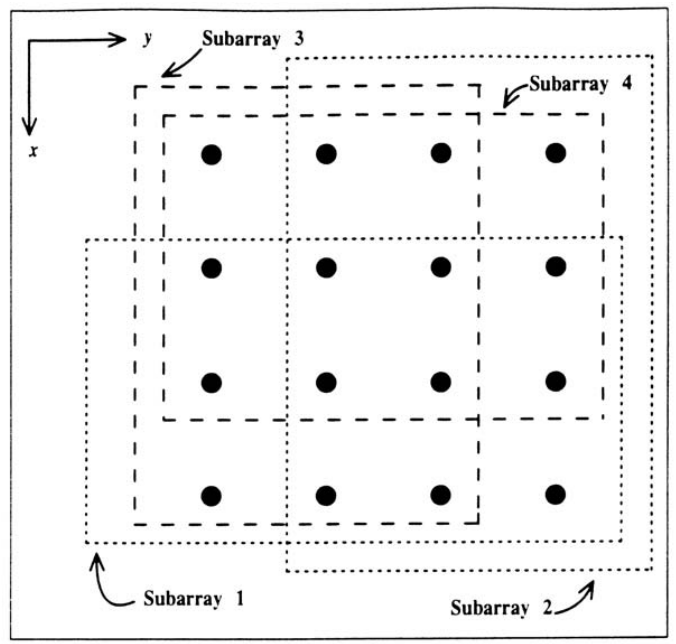
\includegraphics[width=0.8\textwidth]{chapters/figs/fig-5-3}
	\caption{انتخاب زیرآرایه برای \lr{URA} با $M = 4 \times 4 = 16$ عنصر آرایه‌ای (بیشترین هم‌پوشانی در هر دو جهت).}
	\label{fig:5-3}
\end{figure}



فرض کنید $d$ سیگنال بر آرایه می‌تابند. اجازه دهید خروجی‌های آرایه در زمان $t$ به‌صورت یک بردار ستونی $\bm{x}(t)$ روی‌هم‌چیده‌شوند\LTRfootnote{Stacked}، همان‌طور که در بخش \ref{subsec:2-3-2} توضیح داده شد. مانند حالت یک‌بعدی، $d$ سیگنال تابیده با هم ترکیب شده تا یک بردار ستونی $\bm{s}(t)$ را تشکیل دهند. همچنین، فرض کنید بردار نویز جمع‌شونده $\bm{n}(t)$ از یک فرآیند تصادفی با میانگین صفر و ناهمبسته‌ی مکانی با ماتریس کوواریانس مکانی $\sigma_N^2 \bm{I}_M$ گرفته شده است. همان‌طور که در بخش \ref{subsec:3-3-2} بحث شد، سیگنال‌های دریافت شده توسط آرایه را می‌توان به‌صورت زیر بیان کرد:
\begin{equation}
	\bm{x}(t) = \bm{A}\bm{s}(t) + \bm{n}(t)
	\label{eq:5-49}
\end{equation}
که در آن ماتریس هدایت آرایه به‌گونه‌ای فرمول‌بندی شده است که:
\begin{equation}
	\bm{A} = [\bm{a}(\mu_1, \nu_1), \bm{a}(\mu_2, \nu_2), \dots, \bm{a}(\mu_d, \nu_d)]
	\label{eq:5-50}
\end{equation}
و شرط مرکز-متقارن بودن را برآورده می‌کند. رویکرد کار به این صورت است که مسئله \lr{URA} دوبعدی را به دو مسئله یک‌بعدی مستقل تجزیه کنیم \cite{5-1, 5-8}. سپس، می‌توانیم فرکانس‌های مکانی را نسبت به هر آرایه به‌طور جداگانه تخمین بزنیم. فرکانس‌های مکانی $\mu_i$ در جهت $x$ و $\nu_i$ در جهت $y$ نسخه‌های مقیاس‌شده‌ای از کسینوس‌های هادی\LTRfootnote{Direction cosines} متناظر هستند، یعنی:
\begin{equation}
	\mu_i = \frac{2\pi}{\lambda} \Delta_x u_i \quad \text{و} \quad \nu_i = \frac{2\pi}{\lambda} \Delta_y v_i, \quad 1 \leq i \leq d
	\nonumber
\end{equation}

همان‌طور که در بخش \ref{subsec:2-3-2} توصیف شد، \lr{DOA}ها را می‌توان از طریق رابطه زیر یافت:
\begin{equation}
	\phi_i = \arg(u_i + jv_i) \quad \text{و} \quad \theta_i = \arcsin(\|u_i + jv_i\|)
	\nonumber
\end{equation}

مانند الگوریتم \lr{Unitary ESPRIT} یک‌بعدی، برای یافتن این مقادیر، زیرفضای سیگنال و معادله ناورایی باید تخمین زده شوند.

\subsubsection{تخمین زیرفضای سیگنال با مقادیر حقیقی}
\label{subsubsec:5-5-2-1}
به‌عنوان اولین مرحله، زیرفضای سیگنال با مقادیر حقیقی از ماتریس داده به‌دست می‌آید. این کار به‌طور مشابه با حالت \lr{ULA} یک‌بعدی انجام می‌شود، با این تفاوت که ماتریس داده به‌کاررفته در اینجا شامل داده‌های چیده شده به‌صورت ستونی از یک آرایه مستطیلی یکنواخت است. ماتریس داده با مقادیر حقیقی حاصل از تبدیل $\bm{\Gamma}(\bm{X})$ و ماتریس کوواریانس با مقادیر حقیقی $\bm{R}_{xx}$ با استفاده از تبدیل‌های یکانی، مطابق بحث بخش \ref{subsec:5-5-1}، به‌دست می‌آیند. مشاهده شد که این تبدیل یکانی شامل میانگین‌گیری رفت‌وبرگشت نیز هست. فرض کنید $d$ بردار منفرد چپِ غالب از $\bm{\Gamma}(\bm{X}) \in \mathbb{R}^{M \times 2N}$ (رویکرد داده مستقیم) یا $d$ بردار ویژه غالب از $\bm{\Gamma}(\bm{X})\bm{\Gamma}(\bm{X})^H \in \mathbb{R}^{M \times M}$ (رویکرد کوواریانس) به‌صورت $\bm{E}_s \in \mathbb{R}^{M \times d}$ باشد. در این صورت:
\begin{equation}
	\bm{U}_s = \bm{Q}_M \bm{E}_s
	\label{eq:5-51}
\end{equation}
شامل پایه‌ای برای زیرفضای سیگنال تخمینی است. ستون‌های $\bm{U}_s$ در \eqref{eq:5-51} شامل $d$ بردار منفرد چپِ غالب ماتریس داده‌های بسط‌یافته $\bm{Z}$ یا $d$ بردار ویژه غالب از $\bm{ZZ}^H$ هستند. زیرفضاهای با مقادیر حقیقی و مختلط از طریق رابطه \eqref{eq:5-51} به هم مرتبط می‌شوند. در مرحله بعد، دو معادله ناورایی فرمول‌بندی می‌شوند که بعداً به مقادیر حقیقی تبدیل می‌گردند.











\subsubsection{معادله ناورایی با مقادیر حقیقی}
\label{subsec:5-5-2-2}
از آنجا که \lr{URA} به دو جفت زیرآرایه با بیشترین هم‌پوشانی تقسیم شده است، دو جفت ماتریس انتخاب مشابه با رابطه \eqref{eq:5-9} تعریف می‌شوند. ماتریس‌های انتخاب یک‌بعدی برای آرایه‌های خطی یکنواخت در جهت $x$ عبارت‌اند از:
\begin{equation}
	\bm{J}_1^{(M_x)} = [\bm{I}_{M_x-1} \quad \bm{0}], \quad \bm{J}_2^{(M_x)} = [\bm{0} \quad \bm{I}_{M_x-1}]
	\label{eq:5-52}
\end{equation}
به‌طور مشابه، ماتریس‌های انتخاب یک‌بعدی برای آرایه‌های \lr{ULA} در جهت $y$ به‌صورت زیر داده می‌شوند:
\begin{equation}
	\bm{J}_1^{(M_y)} = [\bm{I}_{M_y-1} \quad \bm{0}], \quad \bm{J}_2^{(M_y)} = [\bm{0} \quad \bm{I}_{M_y-1}]
	\label{eq:5-53}
\end{equation}
ماتریس‌های منیفولد آرایه در رابطه ناورایی صدق کرده و می‌توان آن‌ها را به‌صورت زیر بیان کرد:
\begin{equation}
	\begin{aligned}
		\bm{J}_1^{(M_x)} \bm{A}(\mu_i, \nu_i) e^{j\mu_i} &= \bm{J}_2^{(M_x)} \bm{A}(\mu_i, \nu_i) \\
		\bm{A}(\mu_i, \nu_i) (\bm{J}_1^{(M_y)})^T e^{j\nu_i} &= \bm{A}(\mu_i, \nu_i) (\bm{J}_2^{(M_y)})^T
	\end{aligned}
	\label{eq:5-54}
\end{equation}
اکنون با اعمال عملگر $\text{vec}\{\cdot\}$ بر رابطه \eqref{eq:5-54} و استفاده از ویژگی بیان‌شده در بخش \ref{sec:a-1} پیوست، داریم:
\begin{equation}
	\begin{aligned}
		\bm{J}_{\mu 1} \bm{a}(\mu_i, \nu_i) e^{j\mu_i} &= \bm{J}_{\mu 2} \bm{a}(\mu_i, \nu_i) \\
		\bm{J}_{\nu 1} \bm{a}(\mu_i, \nu_i) e^{j\nu_i} &= \bm{J}_{\nu 2} \bm{a}(\mu_i, \nu_i)
	\end{aligned}
	\label{eq:5-55}
\end{equation}
ماتریس‌های انتخاب دوبعدی آرایه \lr{URA} (متناظر با بیشترین هم‌پوشانی) را می‌توان به‌صورت حاصل‌ضرب‌های کرونکر\LTRfootnote{Kronecker products} زیر به‌دست آورد \cite{5-7,5-1}:
\begin{subequations}
\begin{gather}
		\bm{J}_{\mu 1} = \bm{I}_{M_y} \otimes \bm{J}_1^{(M_x)} \quad \text{و} \quad \bm{J}_{\mu 2} = \bm{I}_{M_y} \otimes \bm{J}_2^{(M_x)}
	\label{eq:5-56a}
	\\
	\bm{J}_{\nu 1} = \bm{J}_1^{(M_y)} \otimes \bm{I}_{M_x} \quad \text{و} \quad \bm{J}_{\nu 2} = \bm{J}_2^{(M_y)} \otimes \bm{I}_{M_x}
	\label{eq:5-56b}
\end{gather}
\end{subequations}

این دو جفت ماتریس انتخاب نسبت به یکدیگر مرکز-متقارن\LTRfootnote{Centro-symmetric} هستند، یعنی:
\begin{equation}
	\bm{J}_{\mu 1} = \bm{\Pi}_{m_x} \bm{J}_{\mu 2} \bm{\Pi}_M \quad \text{و} \quad \bm{J}_{\nu 1} = \bm{\Pi}_{m_y} \bm{J}_{\nu 2} \bm{\Pi}_M
	\label{eq:5-57}
\end{equation}
سپس ماتریس هدایت آرایه $\bm{A}$ در دو معادله ناورایی\LTRfootnote{Invariance equations} زیر برای آرایه‌های مستطیلی یکنواخت که ذاتاً مختلط هستند، صدق می‌کند:
\begin{subequations}
	\begin{gather}
		\bm{J}_{\mu 1} \bm{A} \bm{\Phi}_{\mu} = \bm{J}_{\mu 2} \bm{A} \label{eq:5-58a} \\
		\bm{J}_{\nu 1} \bm{A} \bm{\Phi}_{\nu} = \bm{J}_{\nu 2} \bm{A} \label{eq:5-58b}
	\end{gather}
	\label{eq:5-58}
\end{subequations}
که در آن ماتریس‌های قطری با مقادیر مختلط
\begin{subequations}
	\begin{gather}
		\bm{\Phi}_{\mu} = \text{diag}\{e^{j\mu_1}, e^{j\mu_2}, \dots, e^{j\mu_d}\} \label{eq:5-59a} \\
		\bm{\Phi}_{\nu} = \text{diag}\{e^{j\nu_1}, e^{j\nu_2}, \dots, e^{j\nu_d}\} \label{eq:5-59b}
	\end{gather}
	\label{eq:5-59}
\end{subequations}
حاوی اطلاعات زوایای \lr{DOA} دوبعدی مورد نظر برای تخمین هستند.

در مرحله بعد، این معادلات ناورایی با مقادیر مختلط برای \lr{URA} به معادلات ناورایی با مقادیر حقیقی تبدیل می‌شوند، مشابه حالت یک‌بعدی که در بخش \ref{sec:5-5-1} ارائه شد. ماتریس هدایت آرایه دوبعدیِ تبدیل‌یافته را به‌صورت $\bm{B} = \bm{Q}_M^H \bm{A}$ تعریف می‌کنیم. بر اساس دو ویژگی ناوراییِ ماتریس هدایت آرایه دوبعدی $\bm{A}$ در \eqref{eq:5-58}، ماتریس هدایت تبدیل‌یافته $\bm{B}$ در روابط زیر صدق می‌کند:
\begin{subequations}
	\begin{gather}
		\bm{K}_{\mu 1} \bm{B} \cdot \bm{\Omega}_{\mu} = \bm{K}_{\mu 2} \bm{B} \label{eq:5-60a} \\
		\bm{K}_{\nu 1} \bm{B} \cdot \bm{\Omega}_{\nu} = \bm{K}_{\nu 2} \bm{B} \label{eq:5-60b}
	\end{gather}
	\label{eq:5-60}
\end{subequations}
دو جفت ماتریس انتخاب تبدیل‌یافته به‌صورت زیر داده می‌شوند:

دو جفت ماتریس انتخاب تبدیل‌یافته به‌صورت زیر داده می‌شوند:
\begin{subequations}
	\begin{gather}
		\bm{K}_{\mu 1} = 2 \cdot \text{Re}\{\bm{Q}_{m_x}^H \bm{J}_{\mu 2} \bm{Q}_M\}, \quad \bm{K}_{\mu 2} = 2 \cdot \text{Im}\{\bm{Q}_{m_x}^H \bm{J}_{\mu 2} \bm{Q}_M\} \label{eq:5-61a} \\
		\bm{K}_{\nu 1} = 2 \cdot \text{Re}\{\bm{Q}_{m_y}^H \bm{J}_{\nu 2} \bm{Q}_M\}, \quad \bm{K}_{\nu 2} = 2 \cdot \text{Im}\{\bm{Q}_{m_y}^H \bm{J}_{\nu 2} \bm{Q}_M\} \label{eq:5-61b}
	\end{gather}
	\label{eq:5-61}
\end{subequations}

این ماتریس‌های انتخاب با مقادیر حقیقی بدین ترتیب برای به‌دست آوردن معادله‌ی ناورایی با مقادیر حقیقی استفاده می‌شوند.

\subsubsection{تخمین \lr{DOA}}
\label{subsec:5-5-2-3}
فرض کنید ستون‌های $\bm{E}_s$ زیرفضای سیگنال تخمینی با مقادیر حقیقی را پوشش دهند، که همان زیرفضای غالب $\bm{\Gamma}(\bm{X})$ است که در بخش \ref{sec:5-4} مورد بحث قرار گرفت. همان‌طور که پیش‌تر ذکر شد، $\bm{E}_s$ می‌تواند به‌عنوان $d$ بزرگ‌ترین بردار منفرد $\bm{\Gamma}_s(\bm{X})$ (رویکرد داده مستقیم) یا $d$ بردار ویژه‌ی غالب $\bm{\Gamma}_s(\bm{X})\bm{\Gamma}_s(\bm{X})^H$ (رویکرد کوواریانس) محاسبه شود. $\bm{E}_s$ و $\bm{B}$ زیرفضای سیگنال یکسانی را پوشش می‌دهند. بنابراین، یک ماتریس غیرتکین\LTRfootnote{Nonsingular matrix} $\bm{T}_A$ با ابعاد $d \times d$ وجود دارد به‌طوری که:
\begin{equation}
	\bm{B} = \bm{E}_s \bm{T}_A
	\label{eq:5-62}
\end{equation}

جایگذاری رابطه‌ی فوق در \eqref{eq:5-60} منجر به دو معادله‌ی ناورایی با مقادیر حقیقی می‌شود:
\begin{subequations}
	\begin{gather}
		\bm{K}_{\mu 1} \bm{E}_s \bm{\Upsilon}_{\mu} \approx \bm{K}_{\mu 2} \bm{E}_s \in \mathbb{R}^{m_x \times d} \label{eq:5-63a} \\
		\bm{K}_{\nu 1} \bm{E}_s \bm{\Upsilon}_{\nu} \approx \bm{K}_{\nu 2} \bm{E}_s \in \mathbb{R}^{m_y \times d} \label{eq:5-63b}
	\end{gather}
	\label{eq:5-63}
\end{subequations}
که در آن ماتریس‌های با مقادیر حقیقی را می‌توان به‌صورت زیر بیان کرد:





